\newpage
\chapter{Sketch Recognition Techniques}
\label{sec:recognition}

Just as speech and gesture recognition gives us powerful new
interaction avenues, sketch recognition allows a different paradigm
for interacting with computers. This section summarizes strategies for
performing sketch recognition.

An important subset of sketch interpretation is handwriting and
character recognition, which is responsible for converting a person's
handwriting into text. Microsoft's Tablet PC API includes handwriting
recognizers for several languages, as well as symbol and gesture
recognizers for notation systems such as music or mathematics. The
recognition supported by the Tablet PC and other commercial
handwriting recognizers (e.g. Apple's Inkwell~\cite{apple-inkwell}) is
more closely aligned with what Larkin and Simon refer to as
``sentential''~\cite{larkin-diagrams}, as user input is expected to
proceed in a linear, serial fashion. This contrasts with
``diagrammatic'' representations that are expressed over a 2D plane.

Modern pen based computer systems like PDAs or Tablet PCs have
handwriting recognition software that has usable accuracy
rates. Recognition accuracy is typically measured by the deviation
between what the user intended and the machine's
interpretation. \textit{Error tolerance} refers to the recognition
inaccuracy rate a user is willing to accept. One study involving a
modified typewriter found that typists do not notice a word 0.5\%
error rate, 1\% is manageable, but 2\% is
unacceptable~\cite[p. 79]{cole-survey}. It is unclear if there are
similar accuracy thresholds for sketching, though studies have been
conducted for related recognition tasks. For handwriting recognition,
adults find 3\% minimally acceptable, with 1\% considered ``very
good''~\cite{lalomia-recognition-accuracy}. The acceptable accuracy
level depends a great deal on the expected benefit of the task. Users
will accept 20\% error rates if the tool brings greater productivity,
but are intolerant of errors\footnote{It is unclear if the values
described in these articles measure \textit{character} or \text{word}
recognition error rates. Santos \textit{et. al} describe handwriting
recognition error rates of approximately 10\% in terms
of \textit{characters}~\cite{santos-handwriting-recognition}.} when
the perceived benefit is
smaller~\cite{frankish-recognition-tolerance}. Another study examining
user acceptance of hand gesture recognition error rates found users
would tolerate mis-recognition up to 10\% when equivalent keyboard
commands could be employed~\cite{karam-gesture-recognition}.

There are a number of methods for improving recognition. Many PDAs
recognize characters from a constrained symbols set (Latin letters,
Arabic numerals), using different areas of the input surface for
drawing numbers and letters. This approach is not natural, but many
users quickly learn the alternate way of writing. In contrast,
Microsoft's Tablet PC handwriting recognizer allows people to write in
their own handwriting, at any location or angle. Microsoft's
recognizer incorporates a language model (e.g. spelling, grammar) to
guide interpretation.

Recognition is the centerpiece of many software prototypes that
support sketching. Although the research focus of many systems is not
recognition, such systems use automatic interpretation of sketches to
explore new methods of interacting with computers and new ways of
designing~\cite{gross-boe,grundy-maramasketch,lin-denim}. Such
projects rely on reasonably accurate recognizers. Recognition is
therefore a topic that affects nearly all aspects of research on
sketch based systems. For this reason, a substantial portion of this
review is devoted to aspects of sketch recognition. This includes
timing issues, determining what to recognize and how those elements
can be recognized, and interaction issues (see
Table \ref{tab:recognition-topics}).

\begin{landscape}
\begin{table}
\begin{tabular}{p{5cm}| p{2cm} | p{8.5cm}}
\textbf{Topic} & \textbf{Section} & \textbf{Remark} \\
\hline \hline
When to recognize & 
\ref{sec:recognition-when} &
Recognition is powerful but may also distract users from their
task. 
\\ \hline
What to recognize &
\ref{sec:recognition-what} & Sketches may represent objects
(e.g. tables and chairs) and spatial or functional relationships
between those objects (e.g. chairs positioned around table perimeter).
\\ \hline
How much to recognize &
\ref{sec:recognition-how-much} & 
Sometimes only a portion of a sketch need be recognized.
\\ \hline
How to segment &
\ref{sec:recognition-segmentation} &
Sketches contain many different symbols that may overlap. Recognizers
must isolate groups of marks for consideration.
\\ \hline
How to recognize &

\ref{sec:recognition-techniques}, \ref{sec:recognition-patterns}, 
\ref{sec:recognition-3d} &

Many recognition techniques exist, and are reliant on segmentation
methods. \\ \hline

Training recognizers &
\ref{sec:recognition-training} &
In order to recognize something we first need a concept of whatever is
to be recognized. \\ \hline

Managing recognition error &
\ref{sec:recognition-difficulties} &
Recognition sometimes results in inaccurate, ambiguous, or undesired
results.
\\ \hline
Reacting to recognition &
\ref{sec:recognition-action} &
Upon recognition the system must determine how to respond: provide
visual feedback, issue a search query, or take no outward action. \\ \hline

Toolkits for recognition &
\ref{sec:recognition-toolkits} &
Software packages facilitate easier engineering of new recognition
systems.\\ \hline

\end{tabular}
\caption{Topics in sketch recognition}
\label{tab:recognition-topics}
\end{table}
\end{landscape}

\section{When to invoke recognition}
\label{sec:recognition-when}

It is important that sketching systems \textit{aid} design exploration
and not simply \textit{computerize}
it~\cite{negroponte-soft-arc-mac}. For example, a sketch recognition
system might zealously identify parts of the user's drawing as it is
made, replacing the rough sketch with lines or curves. This removes
the opportunity for reflection and re-interpretation that is so
important to the early phases of
design~\cite{schon-reflective,goldschmidt-dialectics,terry-creative-ui}. Premature
recognition may interrupt the designer's flow of thought and interfere
with the task at hand. Instead we may want the computer to eavesdrop
silently, and provide help only when we need it.

A system can provide the user feedback of sketch recognition on
different occasions: (1)~immediately after receiving a single stroke
of input, (2)~as the user works, when feedback may be appropriate,
(3)~only upon request, or (4)~never. Many interfaces attempt immediate
recognition of gestures for invoking commands, such as with marking
menus~\cite{kurtenbach-marking-menus} or PDA device character
input~\cite{palm}. This is commonly called \textit{eager}
recognition~\cite{blostein-diagrams-review}. Other
systems~\cite{gross-ecn-uist,igarashi-suggestive,alvarado-sketchread-uist}
perform recognition in the background, deferring judgment until
adequate information is available. This is termed \textit{lazy}
recognition. Most modern research prototypes take this approach. Last,
some systems wait until the user explicitly requests
recognition~\cite{landay-silk}, or avoid recognition
entirely~\cite{forbus-nusketch-battlespace}. Combinations of these
approaches are common.

One method for identifying sketch input is to sidestep the recognition
process altogether and tell the system what you are about to draw by
choosing from a list or pressing a button. Forbus and colleagues take
this approach as they ``engineer around the need for recognition'' in
their \textit{nuSketch Battlespace} system (nSB) for managing courses
of action for military
commanders~\cite{forbus-nusketch-battlespace}. In order to position an
object such as an armored unit or a movement path, the nSB user
selects an item from a palette of glyphs and draws on the map. The
system interprets the user's ink differently depending on which type
of object is selected. For example when placing military units, the
ink's centroid is taken as the intended location; when defining a
region for those units to defend, the boundary is used.

\section{What should be recognized}
\label{sec:recognition-what}

User input in sketch based applications may be provided in two broad
categories. The first category, often referred to as \textit{digital
ink}, includes stroke timing information. Time data might be used by
sketching applications to determine how quickly the user was drawing,
or when strokes were made relative to one another. Many recognition
algorithms depend on the presence of time information. The second
category describes user input for which time data is unavailable. This
category of sketch input is used by applications that depend on
scanned or photographed
input. Section \ref{sec:recognition-techniques} describes the
differences between these two categories of sketch input from the
recognizer's perspective.

Different kinds of design drawings (``model ink'') in many domains
might be recognized: artistic sketches, study sketches, drawings,
diagrams, schematics, blueprints, and so on. In addition to model ink
comprising those drawing types, user input may be interpreted as a
command (``command ink''). The particular rules about what should be
recognized depends on the domain (architecture or circuit design),
kind of model (floor plan or timing diagram), and other
application-specific requirements. Sketches often contain hand-written
labels or annotations, which are common targets of pen based
recognition.

Diagrams usually have a domain-specific grammar describing how
vocabulary items relate~\cite{lakin-vmacs-89}. For example, boxes may
connect to other boxes via lines, those lines may have arrowheads to
indicate direction. Diagrams are good candidates for recognition
because the various elements and their relations can be described
formally. Table \ref{tab:what} summarizes various recognizable
classes.

\begin{landscape}
\begin{table}
\label{tab:what}
\begin{tabular}{ p{4cm} | p{4.5cm} | p{5.5cm} }
\textbf{``What'' to recognize} & 
\textbf{Examples} & 
\textbf{Remark} \\ 
\hline \hline

Genre &
Mathematical graph, architectural floor plan, web site layout, circuit design &

It may be sufficient to recognize a sketch is of a certain kind
without asking the user. The program could assume the sketch is
in a certain domain.\\ \hline

Characters (writing) & 
Alphanumerics, math symbols & 
Usually with other characters, in words and sentences. \\ \hline

Geometric shapes & 
Dots, lines, rectangles, blobs &
Geometric shapes are often drawn in relation to others. \\ \hline

Spatial features &
A is contained in, is above, is larger than B &
Spatial relations among elements may influence recognition. \\ \hline

Entities &
Domain-specific notation such as diodes, transistors &
Contextual clues can help disambiguate semantics of domain symbols. \\ \hline

Artistic nuance &
Shadows, textures, color &
Ink that modifies an existing element, perhaps suggesting 3D shape. \\ \hline

Commands &
Object selection, delete, copy, move, etc. &
Command ink specifies operations on the drawing. \\ \hline

Intention &
Drawing's function or behavior, e.g. \textit{circuit breaker} & 
Requires detailed domain knowledge and reasoning. \\ \hline

\end{tabular}
\caption{Kinds of elements to be recognized}
\end{table}
\end{landscape}

Artistic sketches and those drawings meant to authentically convey
three dimensional form comprise a different recognition
challenge. Nealen \textit{et. al} (who are concerned with modeling 3D
form) suggest that ``sketching a shape is inverse NPR
(Non-Photorealistic Rendering)''~\cite{nealen-3d-sketch}. Drawings
indicating physical form are not symbolic in the way diagrams are, and
not all drawings of 3D objects are necessarily meant to capture
literal shape. For example, many consumer products come with assembly
instructions featuring simplified diagrams of 3D objects to draw
attention to only those features and relationships relevant for
assembly.

Perhaps the most useful aspect of a sketch is the intention it
captures. The circuit breaker shown in
Figure~\ref{fig:circuit-breaker} probably would not work correctly if
it were manufactured exactly as shown, yet the intent of the drawing
is clear to a person familiar with such engineering
sketches~\cite{stahovich-sketchit-diagram}.

\begin{figure}
\begin{center}
  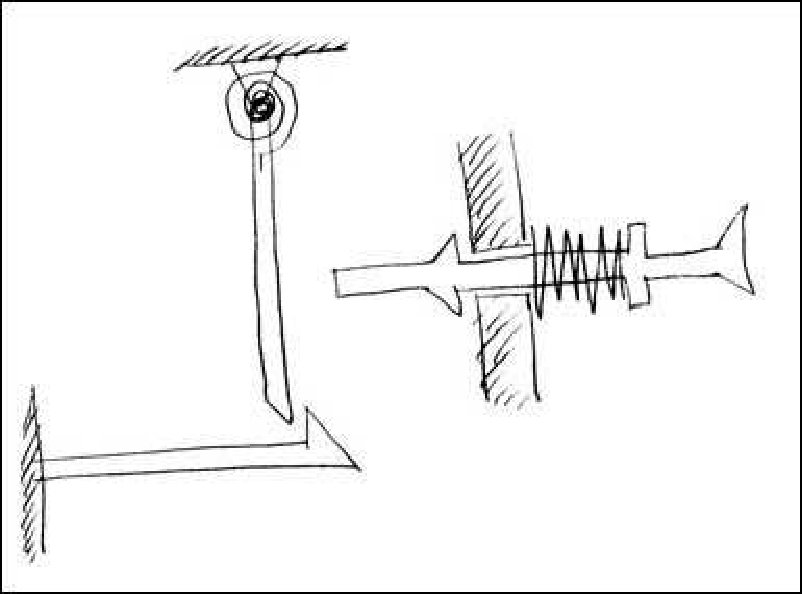
\includegraphics[angle=0, origin=c, width=2.6in]{img/circuit-breaker.pdf}
  \caption{A sketched circuit breaker~\cite{stahovich-sketchit-diagram}.}
  \label{fig:circuit-breaker}
\end{center}
\end{figure}

\section{How much recognition is appropriate}
\label{sec:recognition-how-much}

The nuSketch Battlespace system shows that a sketch based system need
not support recognition at all~\cite{forbus-nusketch-battlespace}. It
aims to enable users to quickly work with spatial data and issue
commands that operate on that data. To support this goal, nSB only
utilizes some properties of the user's ink. For example, the boundary
or center of the ink may be important, but the system need not
recognize the ink as a particular symbol.

Designers often create paper ``storyboards'' for showing high-level
structure or expected behavior without needing to specify
details. DENIM (for web site designers) and DEMAIS (for multimedia
designers) allow users to create such
storyboards~\cite{lin-denim,bailey-demais}. Both these systems
recognize a limited subset of the user's sketch input. Ink that is not
interpreted as belonging to a special set of gestures or symbols is
simply left on the canvas. This allows designers to capture ideas by
sketching naturally without being interrupted by unwanted feedback.

\section{Segmentation and grouping}
\label{sec:recognition-segmentation}

Segmentation and Grouping are related processes of breaking down user
input and finding related ink. Segmentation involves partitioning
undifferentiated sketch input into parts (analogous to identifying
word boundaries in speech recognition~\cite{cole-survey}). Grouping is
the process of forming logical collections of data (analogous to
determining which spoken words compose a sentence).

It is sometimes appropriate to break apart continuous pen strokes into
multiple segments, for example in recognizing cursive writing, or
finding corners in continuous pen strokes. Alternately, it may be
necessary to group related strokes in order to recognize compound
objects such as a triangle drawn with three distinct strokes. To
further complicate matters, there may be a number of reasonable ways
to segment user input~\cite{mankoff-burlap}, based on information such
as pen speed, stroke order, perceptual qualities, domain knowledge or
curvature~\cite{kim-segmentation}. Multi-modal systems may be able to
use additional information such as a user's speech or pointing
gestures to help segment and recognize
sketches~\cite{oviatt-multimodal,anthony-multimodal}. Which
segmentation technique is appropriate depends on what kind of sketch
input the application expects. The technical challenge is simplified
if the system requires users to complete each symbol before moving on
to another, or if each symbol must be drawn using a conventional
stroke order. However, such requirements work against the goal of
supporting unconstrained, fluid sketching.

The following describes three strategies for segmenting and grouping
continuous input strokes. They include the use of temporal data,
perceptual organization, and delimiter-based approaches.

\subsection{Temporal segmentation techniques}
\label{sec:recognition-temporal}

A common and effective method for segmenting ink is to use
time. Temporal data comes in (at least) three flavors. First, we may
look at the order strokes are made. For example, the letter $t$ is
usually drawn with the vertical stroke followed by the horizontal
crossing. Second, timing information for individual $(x,y)$ points tells
us how fast the user was drawing at any given location, which helps
identify corners. Last, a significant delay between individual strokes
may be interpreted as a delimiter between elements, just as a pause in
speech may indicate two distinct sentences.

Even for simple sketches there may be a very large number of possible
ways to segment ink. We can use stroke ordering to reduce
computational complexity of grouping and
recognition~\cite{sezgin-temporal}. Sezgin notes that common
depictions (like stick figures) tend to be drawn using one of a small
set of stroke orderings. However, it is also common for people to
begin drawing one recognizable entity \textit{X}, move to another, and
return to complete \textit{X} later on. For example many people cross
their \textit{t's} and dot their \textit{i's} after writing all
letters of a word. In Sezgin's terms, the user's marks
are \textit{interspersed}.

Another use of time for grouping ink looks at the velocity of the
stylus as the user moves it, to identify locations of interest such as
corners~\cite{sezgin-early-processing,davis-siggraph-tutorial}, or
places where the drawer may be taking extra care to be precise.

A series of strokes with short intervals may constitute a recognizable
entity. For example, people may draw a compound entity like a
television as a square enclosing a circle with a \textit{V}-shaped
antenna along the top. People tend to draw the three parts right after
one another, and then pause to think about what to do next. A
significant pause between pen activity might delimit objects. Such
timeout-based approaches are easy to implement but some users find it
imposes an unnatural feel to the
application~\cite{fonseca-fuzzy-recognition,zeleznik-sketch}.

\subsection{Perceptual organization}
\label{sec:recognition-perceptual-org}

Spatial data can also help with ink grouping. A simple location-based
approach forms groups based on ink proximity: if stroke \textit{A}
overlaps or comes close to overlapping stroke \textit{B}, group them
together. However, this strategy breaks down if distinct entities
overlap.

Gestalt psychologists offer the \textit{laws of perceptual
organization} to explain how people make sense of visual
scenes. Humans perceive scenes not only using what is shown but also
with ``invisible extensions as genuine parts of the
visible''~\cite{arnheim-visthink}. The rules of perceptual
organization include \textit{proximity},
\textit{similarity}, \textit{closure}, \textit{continuation} and 
\textit{common fate}~\cite{kanizsa-gestalt} (see Figure~\ref{fig:gestalt}). 

\begin{figure}
\centering
  \subfigure[] { 
    \label{fig:gestalt-proximity} 
    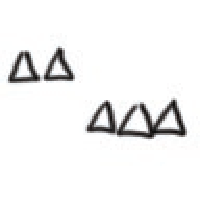
\includegraphics[width=3cm]{img/gestalt-proximity.pdf} 
  }
  \hspace{2mm}
  \subfigure[] { 
    \label{fig:gestalt-similarity} 
    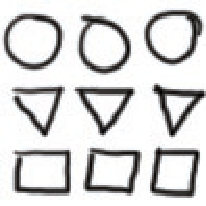
\includegraphics[width=3cm]{img/gestalt-similarity.pdf}
  }
  \hspace{2mm}
  \subfigure[] { 
    \label{fig:gestalt-symmetry} 
    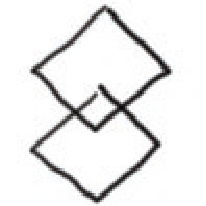
\includegraphics[width=3cm]{img/gestalt-symmetry.pdf}
  }
  \hspace{2mm}
  \subfigure[] { 
    \label{fig:gestalt-continuation} 
    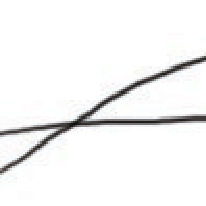
\includegraphics[width=3cm]{img/gestalt-continuation.pdf}
  }
  \hspace{2mm}
  \subfigure[] { 
    \label{fig:gestalt-closure} 
    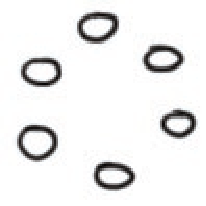
\includegraphics[width=3cm]{img/gestalt-closure.pdf}
  }

\caption{Some principles of perceptual organization~\cite{kanizsa-gestalt}. 
         \subref{fig:gestalt-proximity} Proximity: elements near one
         another are seen as belonging to a
         group. \subref{fig:gestalt-similarity} Similarity: objects
         sharing features such as shape belong in the same
         group. \subref{fig:gestalt-symmetry} Symmetry: two shapes
         symmetric about horizontal and vertical axes, suggesting they
         belong together. \subref{fig:gestalt-continuation}
         Continuation: the simplest explanation is two straight lines,
         not four lines meeting in the
         middle. \subref{fig:gestalt-closure} Closure: A large circle
         emerges from an arrangement of smaller circles.}
\label{fig:gestalt}
\end{figure}

Perceptual organization supports grouping at many levels. At a
low-level, we can use perceptual rules to analyze the relationship
among individual ink strokes to find plausible groupings for
recognition. Mahoney and Fromherz show how perceptual organization
rules can reduce the number of plausible stroke groupings into a
ranked list of groups, which helps improve recognizer
efficiency~\cite{mahoney-sketching-issues}. For example, an object may
be drawn on top of background elements, as illustrated by the stick
figure and horizon from Figure~\ref{fig:cloud}. Because the horizon
has strong continuity from the left to the right of the stick figure,
it is plausible the two halves should be grouped. The marks forming
the stick figure are in close proximity, and share similar sizes,
suggesting they may form a logical whole.

PerSketch and ScanScribe explore how perceptual organization rules can
be used on a number of
levels~\cite{saund-persketch,saund-perceptual}. Drawings are analyzed
in a manner approximating Marr's three-stage visual information
processing theory~\cite{marr-visual-infoprocessing}. In the early
phase, ink is broken into ``elemental curve fragments'' called Prime
objects (Primitive objects in ScanScribe). In the middle stage, Prime
objects are put into plausible groups using perceptual organization
rules. These groups are called Composite objects. Composite objects
may include Primes as well as other Composites. In the last stage,
domain rules are applied to combinations of Composite objects,
identifying which combinations of composite objects are reasonable
according to the subject matter (e.g. chemical modeling or electrical
engineering).

Gennari \textit{et. al} propose a segmentation approach based on
finding dense areas of ink and areas where the perceptual qualities of
the ink changes~\cite{gennari-parsing}. The Gennari system analyses
input as the user draws, calculating features such as ink
density. This approach is designed to work for node-and-edge diagrams
whose symbols do not overlap.

\subsection{Context-aware segmentation}

Particular aspects of the domain's graphical language may afford the
opportunity to use clever strategies for segmenting ink. This section
describes two methods for forming groups of marks by analyzing ink.

\begin{figure}
\begin{center}
  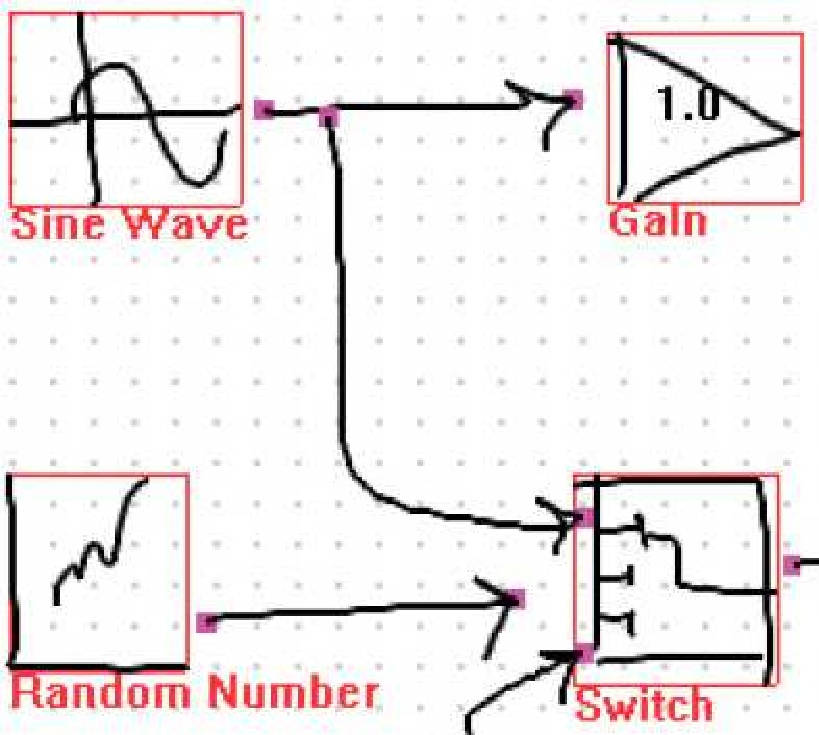
\includegraphics[angle=0, origin=c, width=2in]{img/simusketch.pdf}

  \caption{SimuSketch exemplifies delimiter-based, multi-phase parsing
  of sketches. The first stage identifies arrows as delimiters. In the
  second stage, clusters of remaining ink are recognized as domain
  symbols. }

  \label{fig:simusketch}
\end{center}
\end{figure}

Kara and Stahovich's SimuSketch is a sketch based interface for
creating graphical node-and-edge network diagrams in the Simulink
application. Simulink supports users in simulating dynamic systems
with a visual programming approach wherein boxes (nodes) represent
functions or processes, and connectors (edges) represent inputs and
outputs. SimuSketch looks for
\textit{markers} in the input sequence---easily identifiable 
symbols used to group other (non-marker) ink. In particular,
SimuSketch looks for edges between nodes (see
Figure~\ref{fig:simusketch}). 

Shilman's work on parsing handwritten notes incorporates context
awareness for discerning the structure of a sketched
document~\cite{shilman-discerning-structure} (see
Figure~\ref{fig:shilman-text-or-drawing}). Shilman's algorithm
integrates two related tasks in document analysis. The first challenge
is to discern marks as either writing or pictures. The second
challenge is handwriting layout analysis--grouping ink that has been
identified as writing into compound entities such as words, sentences,
and paragraphs. By combining these two processes,
Shilman \textit{et. al} can perform a limited feature-based
recognition on ink in order to test if it is text. The intuition is
that ``if you look at a page of ink with squinted eyes or from a
distance, you can distinguish writing from drawing by its regular,
linear structure.''  This approach uses features such as stroke length
and curvature as well as information derived from the spatial and
temporal relationship between fragments of ink. Marks are labeled as
either `text' or `drawing' using these local and global features with
a decision tree classifier.


\begin{figure}
\centering
\subfigure[]
{
    \label{fig:shilman-text-or-drawing-1}
    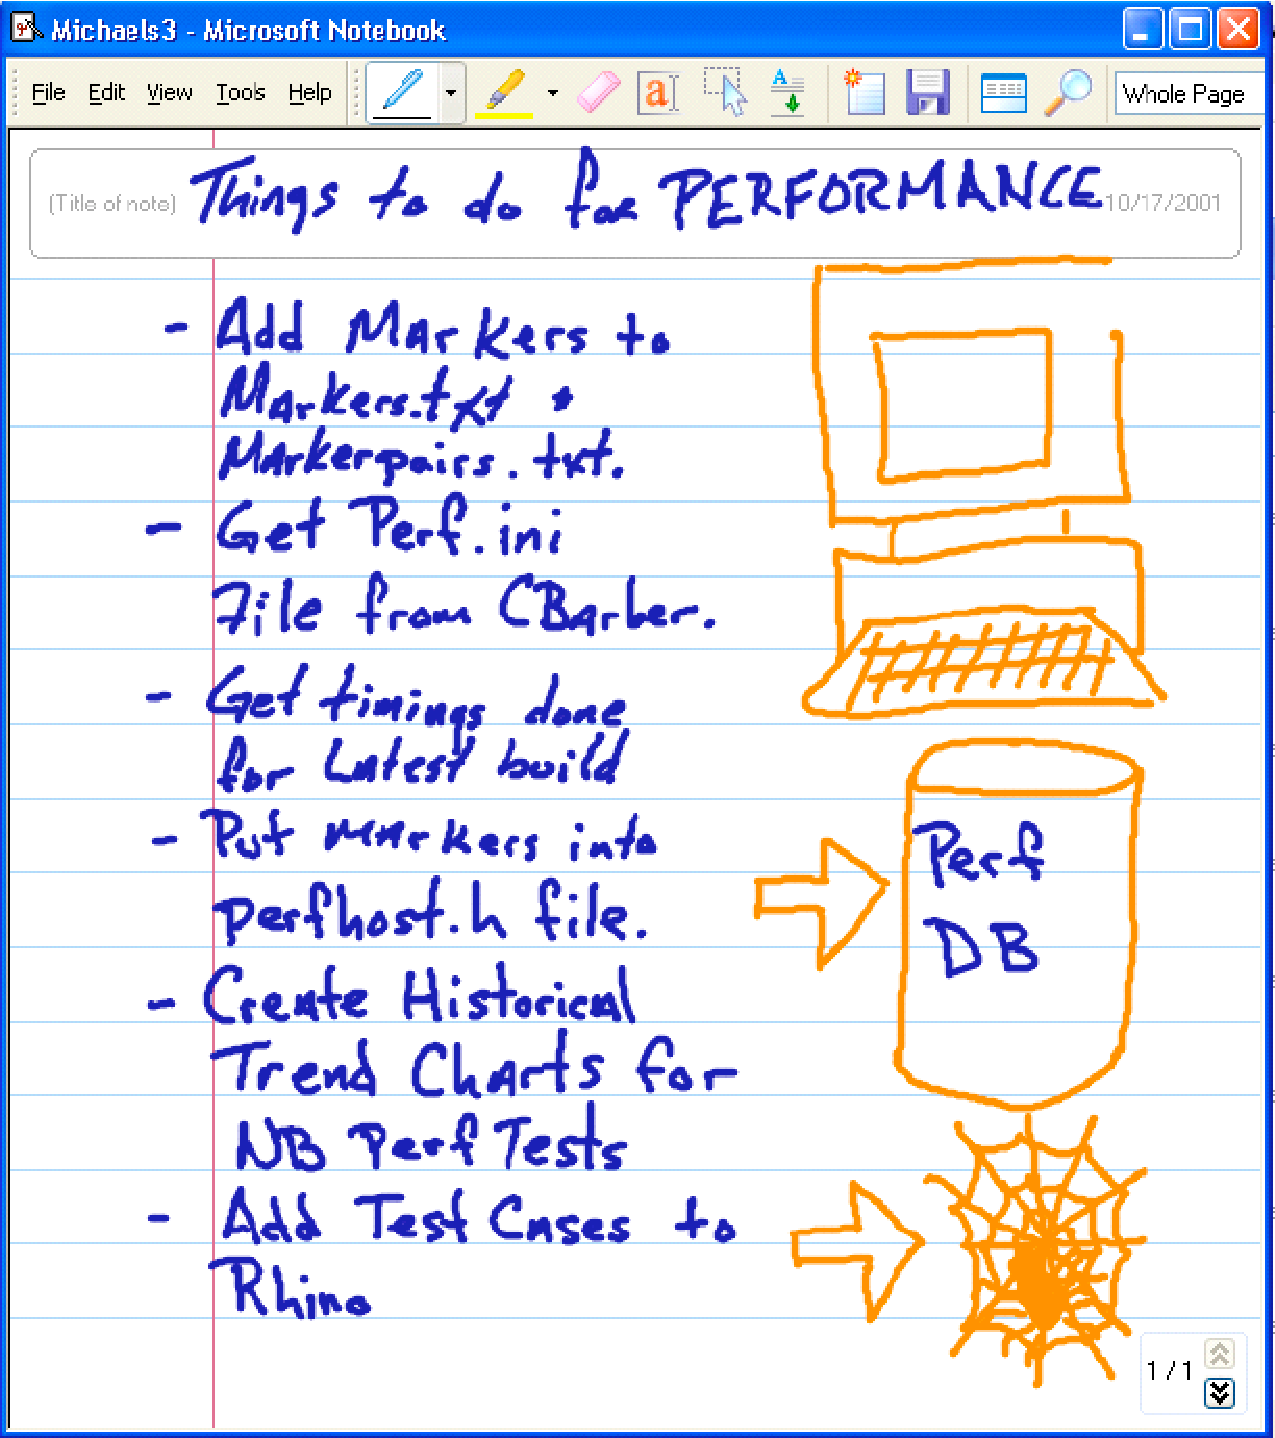
\includegraphics[origin=c, width=4cm]{img/shilman-1.pdf}
}
\hspace{1cm}
\subfigure[]
{
    \label{fig:shilman-text-or-drawing-2}
    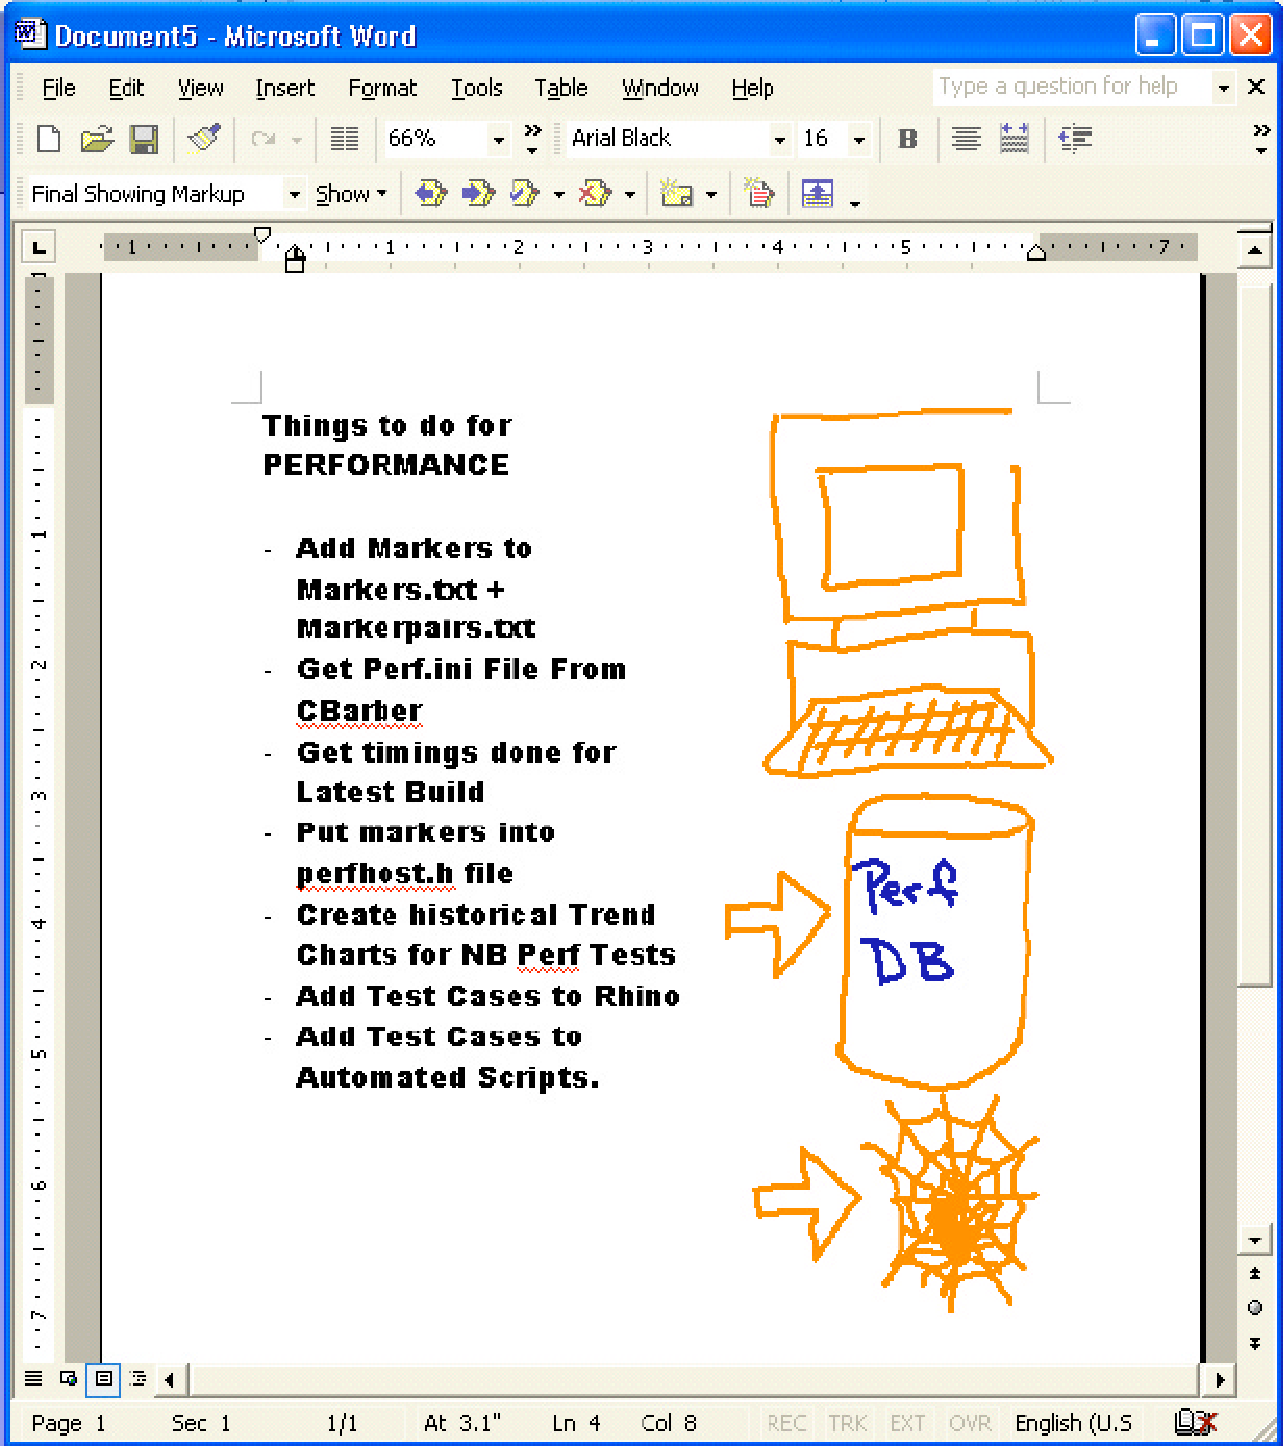
\includegraphics[origin=c, width=4cm]{img/shilman-2.pdf}
}

\caption{Analysis of hand-written notes discern writing
                  from drawings. Left: the original electronic
                  document. Right: the same document after handwriting
                  has been
                  recognized~\cite{shilman-discerning-structure}.}

\label{fig:shilman-text-or-drawing}
\end{figure}

\section{Overview of recognition techniques}
\label{sec:recognition-techniques}

This section gives a brief overview of various approaches for
performing sketch recognition.

Regardless of the input device, we identify two broad categories of
sketch recognition: \textit{on-line} and \textit{off-line}. On-line
recognition is analogous to your friend watching you sketch. Your
friend may see how fast you make a stroke, in which order you make
marks, and perceive what you say and how you gesture as you
sketch. Interpretation happens as the drawing is made. Off-line
recognition is analogous to your friend seeing your sketch for the first
time after you have finished it. Recognition happens after the drawing
is complete, irrespective of the order or speed strokes were
made. While off-line recognizers only have access to the finished
drawing, on-line recognizers potentially have access to data such as
pen pressure, time, speech, and gesturing.

Pen input is generally captured as a sequence of time-ordered 2D
coordinates. Other data such as pressure or (in a multi-user
environment) user identity may be available depending on the input
hardware. A single sequence of ink captured while the stylus is
touching the drawing surface is commonly called a \textit{stroke}.

On-line recognition strategies are further divided in two categories:
single-stroke and multi-stroke recognizers. Single-stroke recognizers
are appropriate for tasks such as interpreting freehand
gestures. Single-stroke approaches are simpler to implement than
multi-stroke strategies because user input is clearly divided into
pieces. This process could be relatively simple: a multi-stroke
recognizer might simply expect multi-stroke objects to be drawn in a
prescribed fashion. Or, multi-stroke recognizers might be more
complex, for example hypothesizing which individual strokes (or
segments of strokes) belong together, using Markov models or Bayesian
Networks to aid hypothesis testing.

We need some way of representing the \textit{entities} for
recognition. By ``entity'' we refer to classes that may be recognized:
boxes, lines, chairs, AND-gates, and so on (see also Table
\ref{tab:what}). The examples a recognition system has learned are
called \textit{classes}, and user's input are
\textit{candidates}. Three methods of presenting classes are covered
here: hard-coded, visual example, and textual description. Particular
instances of these methods are described later.

\subsection{Hard-coded recognizers}

One common approach is to hard-code recognition routines directly. For
simple or limited graphical vocabularies this may be appropriate. A
circle (or a zero, or the letter 'O', or the sun, etc.)  can be
recognized with a short program looking for input points that are
roughly equidistant from the stroke's centroid. However, ad-hoc,
hard-coded recognizers are difficult to maintain and extend. For
example, if we wished to extend our circle recognizer to interpret a
sun with rays of light coming out of it, we would have to also
recognize lines, then coordinate the recognizer to consider those
particular lines together with the circle, and ensure that the lines
are positioned and angled correctly. Further, sketch recognition
applications must be able to discern different kinds of elements. The
recognizers for each of these elements may conflict. A new recognizer
may cause an existing recognizer to stop working correctly, leading to
maintenance, debugging, and testing problems.

\subsection{Visual matching}
\label{recognition-library}

Another strategy for representing classes is to create a library of
drawn examples. Some techniques that use this approach are the Ledeen
recognizer~\cite{newman-sproull-graphics-2}, the Rubine
recognizer~\cite{rubine-recognizer}, Quill (based on
Rubine)~\cite{long-quill-chi}, Kara's
recognizer~\cite{kara-recognizer-cg}, and the \$1
Recognizer~\cite{wobbrock-dollar}. The accuracy of some of these
approaches can be improved if multiple training examples are
provided. Other techniques require only a single training example.

Some of these approaches are \textit{feature-based}. Such strategies
compute properties such as stroke length, stroke path, minimum or
maximum angle, or aspect ratio. A user's candidate entity is compared
with classes using these features. An alternate approach is to treat
visual examples as \textit{graphical templates}, where candidates and
classes are compared using some form of distance function.

User tests of recognition systems employing visual libraries commonly
include 30 or fewer classes~\cite[page 13]{kara-recognizer-cg}. For
many applications a database of that size is appropriate. It is
unclear how large these database can be: on one hand, human users have
limited ability to recall how uncommon symbols must be drawn; on the
other hand, recognition systems must search its (potentially
extensive) library for matches. The larger the database, the greater
probability of matching multiple classes, possibly leading to
ambiguity.

Library-based recognition schemes differ in how quickly the algorithm
searches its class database. Quill and the Rubine Recognizer compare
user input to each symbol, while other strategies (such as Kara's
recognizer) use efficient methods that exclude large portions of the
library before performing computationally intensive comparisons on the
remaining symbols. All of the methods discussed in the previous
paragraph provide interactive performance on the target hardware. For
example, the 1\$ recognizer produced results within about one second
using a consumer-grade PDA from 2006 with 16 symbols in the
recognition library~\cite{wobbrock-dollar}.

\subsection{Textual description}

Classes may be described textually using a programming
language~\cite{pasternak-adik,bimber-sketch-bnf,costagliola-xpg,hammond-ladder}. These
notations have two primary strengths. First, humans can read them. The
television symbol described in Section~\ref{sec:recognition-temporal}
may be described with natural language as ``a square with a slightly
smaller circle positioned at its center.'' A formal symbolic language
for that statement is still quite legible (assuming one understands
the function semantics):

\begin{verbatim}
      (define television 
              (and (centered square circle)
                   (slightly-smaller circle square)))
\end{verbatim}

Another strength of this kind of notation is that it allows the
developer to describe entities at a level of abstraction that
accommodates variability between entity
instances. An \textit{abstract} triangle is a three-sided,
two-dimensional convex shape whose internal angles sum up to
180\degree. A \textit{particular} triangle may have side lengths of 3,
4, and 5, and be oriented so that its long edge is horizontal. We may
define triangles and other entities as abstractly or concretely as the
language allows.

\subsection{Managing ambiguity}
\label{sec:recognition-managing-ambiguity}

Futrelle's classification scheme of types of ambiguity in diagrams
includes two high-level categories: lexical and structural
ambiguity~\cite{futrelle-ambigutiy}. Lexical ambiguity refers to the
``word'' level, when the meaning of a particular symbol is in
question. Structural ambiguity refers to confusion arising from the
composition of symbols.

Shilman augments this scheme with two additional types of ambiguity
that arise in sketch recognition: label and attribute
ambiguity~\cite{shilman-parsing}. Label ambiguity is present when the
symbol's identity is unclear. For example, a quickly drawn rectangle
might be interpreted as a circle. Attribute ambiguity refers to the
features of a sketched element: the exact location of a quickly drawn
rectangle's corner may be unclear.

Two sketching systems that focus on managing ambiguity at different
stages of user interaction are BURLAP and SketchREAD. A technique
built into BURLAP~\cite{mankoff-burlap} addresses domain independent
ambiguity management at the GUI toolkit level, while
SketchREAD~\cite{alvarado-sketchread-uist} offers a method for using
domain knowledge to disambiguate domain symbols.

BURLAP is a calligraphic application based on SILK~\cite{landay-silk}
that enables people to draw user interfaces. As the user draws, BURLAP
forms a list of plausible interpretations. At some point the system
may need to pick one interpretation.  Mankoff \textit{et. al} call
this process \textit{mediation}, performed by agents
called \textit{mediators}. Some mediators may engage the user by
displaying a pick-list of choices or visually indicating the
ambiguity. Other mediators automatically execute and do not involve
the user.

BURLAP exemplifies a framework for mediating ambiguity in
recognition-based interfaces called OOPS~\cite{mankoff-oops}. OOPS
consists of a library of error correction and ambiguity management
techniques that work with existing GUI toolkits at the input-event
level.

Alvarado and Davis's SketchREAD system demonstrates a technique for
modeling recognition ambiguity~\cite{alvarado-sketchread-uist}. The
SketchREAD application is a domain-independent sketching tool. It
accepts a textual description of classes to learn to recognize in a
particular domain~\cite{hammond-ladder} (see
Section~\ref{sec:recognition-training}). SketchREAD uses Bayesian
Networks to reason about the user's input based on domain
understanding~\cite{alvarado-dynamic-bayes}.

Bayesian Networks also allow us to encode relations of compound
objects that can further influence the belief in a hypothesis.
Alvarado and Davis give an example from a circuit design
application~\cite{alvarado-sketchread-uist}. A diode is depicted as a
triangle with a line tangent to one of the corners and parallel to the
opposing triangle edge (see Figure~\ref{fig:diode}). A person
typically draws a triangle first. The system calculates the
probability $P(triangle)$ that the marks depict a triangle. In circuit
diagrams, triangles are strongly correlated with diodes, so at this
point there is a \textit{partial hypothesis} that the person is
drawing a diode. Next, when the diode's line is drawn the system
calculates $P(line)$. Because a diode consists of a triangle and a
line, the Bayesian Network tests the hypothesis that the drawing is a
diode by calculating the joint probability of the triangle and line
interpretations. Even if one of the two parts (triangle or line) were
drawn sloppily, the higher-level hypothesis \textit{diode} can guide
us to a meaningful interpretation. If additional information is
present (such as connecting wires), additional belief values can be
used to support or reject the hypothesis that the drawing depicts a
diode.

A nice property of this recognition strategy is that it supports
efficient re-interpretation on an ongoing basis as the user continues
to work. The system endeavors to make sense of each new input stroke,
making use of established interpretations and associated
probabilities. While na\"ive systems may exhaustively test all
possible interpretation hypotheses, SketchREAD's hypothesis pruning
enables the system to test only the most likely
interpretations. SketchREAD's interpretation speed scales roughly
linearly with the number of strokes, compared to the exponential
runtime used by some other approaches.

\begin{figure}
\begin{center}
  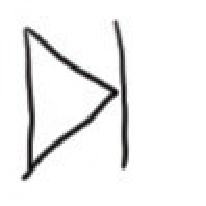
\includegraphics[angle=0, origin=c, width=0.7in]{img/diode.pdf}
  \caption{A diode is drawn as a triangle with an adjacent line.}
  \label{fig:diode}
\end{center}
\end{figure}

\section{Pattern recognizers}
\label{sec:recognition-patterns}

Various methods have been investigated for performing recognition of
sketch input. The methods covered have been known variously as
character recognizers, glyph recognizers, and pattern
recognizers. They operate on isolated strokes or segments of strokes
and do not perform higher-level reasoning based on domain semantics or
context.

All these recognition approaches work using the same general strategy,
and although each has its own strengths and weaknesses, no single one
is best for everything. The general strategy has not changed since the
earliest on-line character recognition
systems~\cite{groner-grail-recognizer,newman-sproull-graphics-2}. The
first step is to learn a dictionary of \textit{classes}. These serve
as instances of the elements the recognizer can handle. The
recognition system converts user input into \textit{candidates}. The
candidate is then compared to classes in the dictionary, producing a
similarity metric for each comparison. Sketch based applications can
use higher-level methods to reason about the most likely choice or
choices. Alternately, the best match from the low-level recognizer
might be used.

While the recognition strategies described below share a high-level
strategy, they differ in how they represent candidates and classes and
how they are compared.

\subsection{Ledeen recognizer}

The Ledeen character recognizer is efficient and easily
trained~\cite{newman-sproull-graphics-2}. User input is scaled to fit
inside a three-by-three grid of nine cells. Each stroke's starting
cell is noted, and each stroke's path through the grid is
encoded. This approach accommodates multiple stroke input but does not
specify how multiple strokes should be grouped to be considered
together. Newman and Sproull suggest considering multiple strokes
together if less than half a second of latency separates strokes.

Some user input is not easily handled with this scheme. For example,
straight vertical or horizontal lines would require scaling one
dimension significantly more than another, leading to an unreliable
path order. Dots also give this approach trouble. Problematic strokes
like dots and vertical or horizontal lines are recognized by
special-case algorithms instead of the 3$\times$3 grid approach. GRAIL
employed a multi-stroke, context-sensitive recognition strategy very
similar to the Ledeen recognizer~\cite{groner-grail-recognizer}.

\subsection{Rubine Recognizer}
\label{sec:recognition-rubine}

Rubine's feature-based recognition approach was demonstrated by a
system called GRANDMA (Gesture Recognizers Automated in a Novel Direct
Manipulation Architecture). The features involve geometric properties
of single strokes such as start/end locations, total gesture length,
sine/cosine of initial angle, and so on. Each feature must be
calculable in constant time to ensure efficiency.

Some features are more effective than others for classifying a given
symbol. If a number of examples are provided (typically 15 or more
produce good results), the trainer uses linear discriminant analysis
to determine the most effective features for classifying a particular
entity.

Rubine's work was extended with a recognition system called gdt (later
renamed Quill)~\cite{long-quill-chi}, and added several feature types
such as aspect ratio and curviness. Quill was incorporated into
SATIN~\cite{hong-satin}, a toolkit for building sketch based
applications.

\subsection{Kara's Recognizer}

A recognition technique developed by Kara and
Stahovich~\cite{kara-recognizer-cg} differs from stroke-oriented,
feature-based approaches such as Rubine's. Instead, it compares the
spatial distance between down-sampled bitmap representations of
symbols. Kara's recognizer does \textit{not} rely on geometric
features like corners, angles or lines, and operates on input
regardless of temporal information. Further, it accommodates
multi-stroke entities as easily as single-stroke entities.

The technique first applies a polar coordinate transformation about a
cleverly chosen pivot point. Input is incrementally rotated from
-$\pi$ to +$\pi$ radians and compared with a class entity to determine
a rotation that best aligns two symbols. This ``pre-recognition'' step
helps exclude unlikely matches.

After rotating the user's input the algorithm creates an
\textit{n}$\times$\textit{n} down-sampled bitmap (\textit{n}=48 works
well). Next the recognizer applies four spatial distance classifiers
to compare user input against known classes. The results of each
classifier are converted into comparable forms and combined to produce
a single recognition value describing the similarity between the user
input and classes.

\subsection{Cali Recognizer}

Fonseca \textit{et. al's} non-trainable Cali recognizer can identify
geometric shapes at any angular orientation or aspect
ratio~\cite{fonseca-caligraphic,fonseca-fuzzy-recognition}. These
shapes may consist of any number of strokes, as they are segmented
based on a timeout (see Section~\ref{sec:recognition-temporal}). To
identify the shape (triangle, cross, etc.) Cali first finds geometric
properties based on the input: the convex hull, the largest triangle
and quadrilateral inscribed inside the hull.  Additional geometric
properties are calculated based on these shapes, including areas and
perimeter values and aspect ratios. These values are then used to
search through prior statistical data regarding the shapes to be
recognized. This approach uses fuzzy logic to determine membership in
statistical equivalence classes. For example the recognizer for the
shape ``Line'' reports true if the input's aspect ratio ``is very
thin''.

A trainable variant of Cali compared several learning algorithms for
building the statistical equivalence classes: K-nearest neighbors,
inductive decision trees, and Naive Bayesian Networks. Testing showed
Naive Bayesian Networks the easiest to train with the best recognition
rates.

\subsection{\$1 Recognizer}

The \textit{\$1 Recognizer}~\cite{wobbrock-dollar} is notable because
of its ease of use, algorithmic elegance and power. This technique is
designed for use on PDA-like devices that accept pen based, gestural
input for characters and commands. The \$1 Recognizer requires only a
single training example to be effective. Users may easily create their
own gestures---it is trainable on the fly.

The algorithm processes candidate and class input the same way. It
begins by resampling input into a number of points (n=64 was found
adequate). This enables \$1 to compare strokes of different sizes and
drawing speeds. Next, the input is rotated so the angle formed by the
input's centroid and initial point is 0\degree. After rotation the
input is scaled non-uniformly to fit inside a square. Like the Ledeen
algorithm, the \$1 Recognizer must handle certain classes of input
(e.g., straight lines) differently because scaling the input
non-uniformly would distort it too much. Last, the candidate is
compared to each class in the dictionary by summing the error of
corresponding points.

\subsection{Graph matching techniques}
\label{sec:recognition-graph}

\begin{figure}
\begin{center}
\subfigure[] {
  \label{fig:llados-graph-1}
  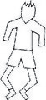
\includegraphics[origin=c,height=1.0in]{img/llados-1.pdf}
}
\subfigure[] { 
  \label{fig:llados-graph-2}
  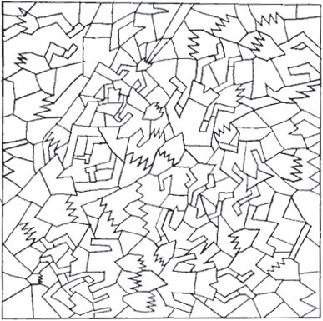
\includegraphics[origin=c,height=1.7in]{img/llados-2.pdf}
}
\subfigure[] { 
  \label{fig:llados-graph-3}
  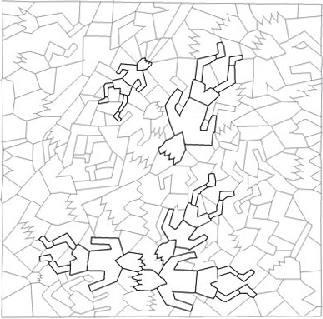
\includegraphics[origin=c,height=1.7in]{img/llados-3.pdf}
}
\caption{Example of graph-based pattern matching~\cite{llados-rag}. An
  example pattern is shown in \subref{fig:llados-graph-1}. The complex
  test image in \subref{fig:llados-graph-2} contains several
  distorted, scaled and rotated instances of the pattern. Portions of
  the example pattern found in the test image within acceptable error
  tolerance are shown in \subref{fig:llados-graph-3} with thick
  lines.}
\label{fig:llados-graph}
\end{center}
\end{figure}

The techniques discussed earlier are best used for on-line recognition
because they require timing data regarding stroke path (e.g. Ledeen's
approach) or where strokes begin and end (e.g. \$1 or Kara
recognizers). But on-line recognition is not always possible. A
designer may scan a paper sketch and expect to use it as the basis for
further work. In such cases, off-line recognition might be
employed. Graph-based recognition techniques are commonly used for
this purpose in the document analysis and engineering diagram research
community.

The first step in graph-based off-line recognition is to convert the
input image from a raster to a vector
representation~\cite{tombre-vectorization}. Vector endpoints and
junctions form graph nodes, and edges represent lines between
them. Because graph nodes contain additional information such as
$(x,y)$ position, these structures are called \textit{attributed
relational graphs}.

A full drawing's corresponding graph can be searched for identifiable
portions, or subgraphs using \textit{subgraph isomorphism}
algorithms~\cite{lee-graph-matching}. Llad\'{o}s has proposed an
heuristic technique for error-tolerant pattern matching using subgraph
isomorphism~\cite{llados-rag}. For example, suppose we are interested
in finding the pattern shown in Figure~\ref{fig:llados-graph-1} in the
test image shown in Figure~\ref{fig:llados-graph-2}. After converting
both the example pattern and the test image to attributed relational
graphs, this technique begins searching through the test image graph
for sequences that resemble the example pattern's graph. When this
algorithm finds a near match, it employs edit operations on the test
image graph to force an exact match. Recognition confidence is
measured in terms of how much the observed graph must be edited in
order to match the expected graph. As shown in
Figure~\ref{fig:llados-graph-3}, the approach is rotation and scale
invariant and tolerates some degree of distortion.

\section{Recognition of 3D scenes}
\label{sec:recognition-3d}

Although many sketches represent abstract entities that lack physical
form (e.g. UML diagrams), many others have physical, three-dimensional
interpretations. In this section, ``recognition'' refers to
reconstructing 2D sketch input as 3D models. In this sense the
recognition is syntactic (e.g. identifying a rectangular
parallelepiped) rather than semantic (e.g. identifying a shoe
box). Reconstruction of 3D scenes has been studied in the robotics and
computer vision community as well as by CAD researchers.

3D recognition is essentially ``reverse projection''. The strokes on
the drawing surface provide $(x,y)$ data but not depth
$(z)$~\cite{lipson-correlation}. Because $z$ could take on any value
there are an infinite number of ways the 2D drawing could be turned
into a 3D model. Fortunately knowledge of solid geometry restricts the
possible interpretations: the surface of a 3D object can not pass
through itself, so any interpretation that involves self-intersecting
surface planes is invalid. There are many ways to compute particular
$z$ values for sketched 3D models. Analytic approaches include line
and junction coding~\cite{clowes-seeing-things,huffman-nonsense} and
solving linear equations~\cite{grimstead-3d-linear-system}. Other
approaches attempt to fit sketch input to likely constructions such as
primitive 3D structures such as cylinders~\cite{wang-3d-sketch}, or by
finding likely geometric constraints like parallelism and
symmetry~\cite{shpitalni-curve-fitting}. Many 3D sketch recognition
systems employ a combination of these approaches.

People can recognize sketches as long as they are made from a familiar
vocabulary. We also make inferences about 3D shape based on 2D
perceptual qualities such as parallelism, right angles, and alignment
to primary axes. Further, drawings of 3D objects often use shading to
show shadows and contours. Frequently when people draw a 3D object,
they draw only the visible contours, leaving the rest to the
imagination. It is not difficult to look at a box and be able to
``see'' the edges and corners that are obscured by the solid geometry
(although the imagined edges might in fact be wrong). Some have
developed heuristic methods for hidden-line
inference~\cite{mumford-hidden-line,karpenko-smoothsketch} that
``reconstruct'' a 3D object without access to a complete 2D
wireframe. A wireframe model shows edges in a ``see-through'' view;
hidden lines are shown through surfaces.

\begin{figure}
\begin{center}
  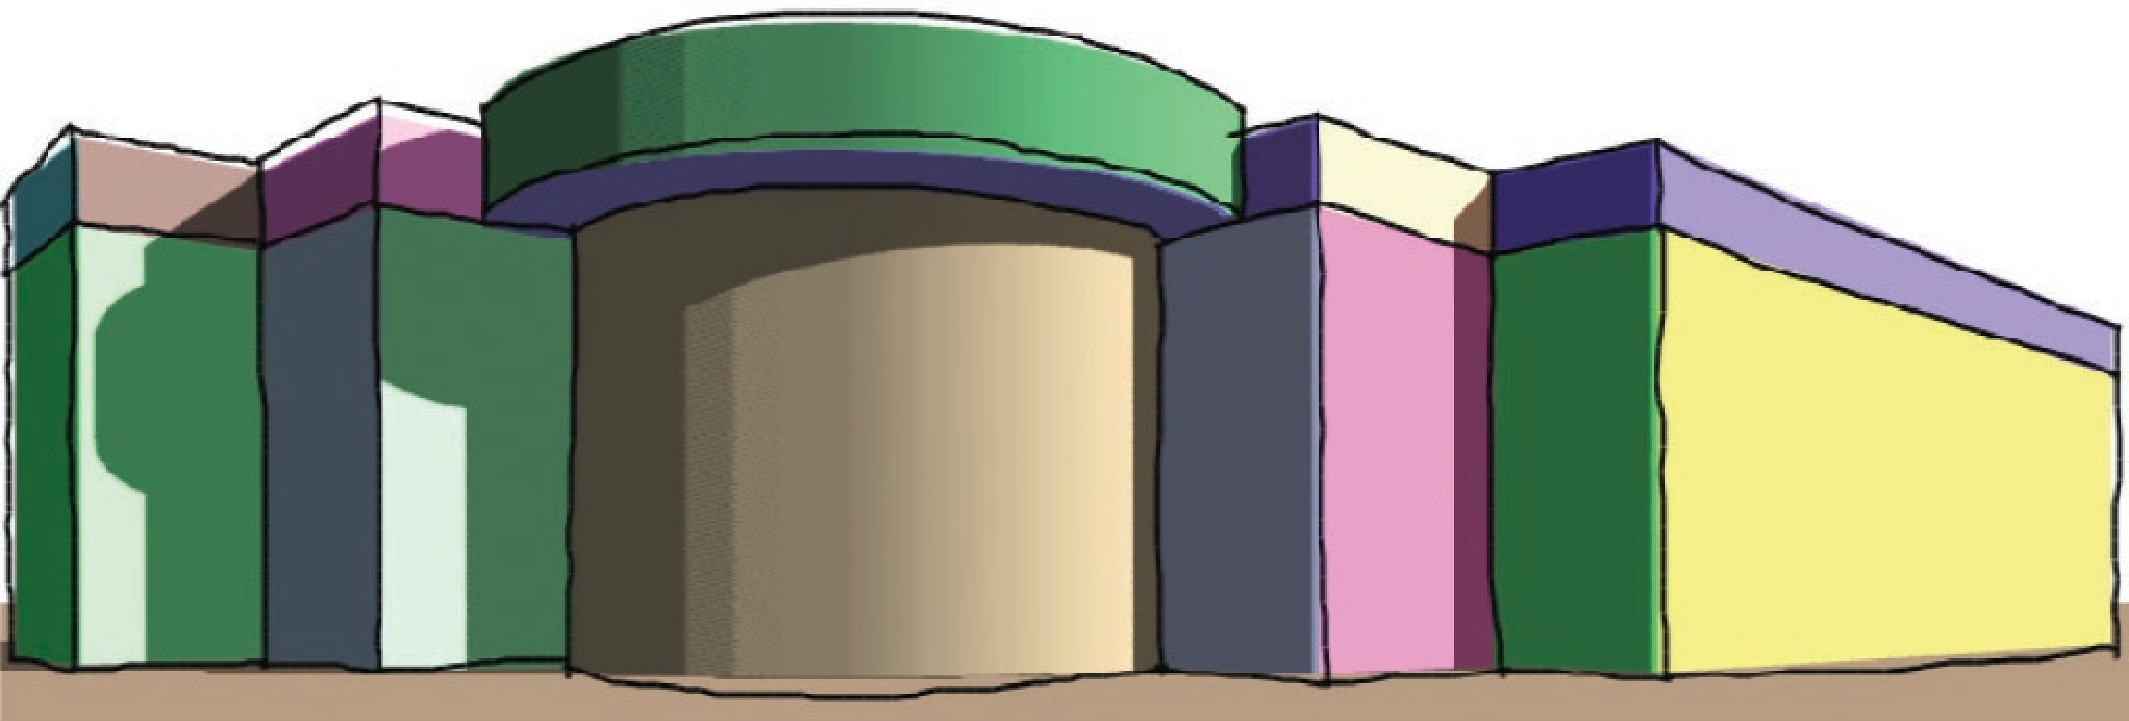
\includegraphics[width=3in]{img/sketching-reality.pdf} \caption{``Sketching
  reality'' allows users to create 2.5D architectural models by
  sketching~\cite{chen-sketching-reality}.}  \label{fig:sketching-reality}
\end{center}
\end{figure}

Design software need not reconstruct full 3D models to be
useful. Instead, the recognition system could build a 2.5D
interpretation of a 2D sketch. A 2.5D model contains depth information
only for geometry visible from a single vantage point, so the
recognition system is relieved of the difficult task of inferring the
full 3D structure. Recent work from Microsoft Research Asia
demonstrates an interactive 2.5D recognition and rendering
system~\cite{chen-sketching-reality}. Figure~\ref{fig:sketching-reality}
shows sample output of this approach.

\subsection{3D Curve Analysis}

\begin{figure}
\begin{center}
   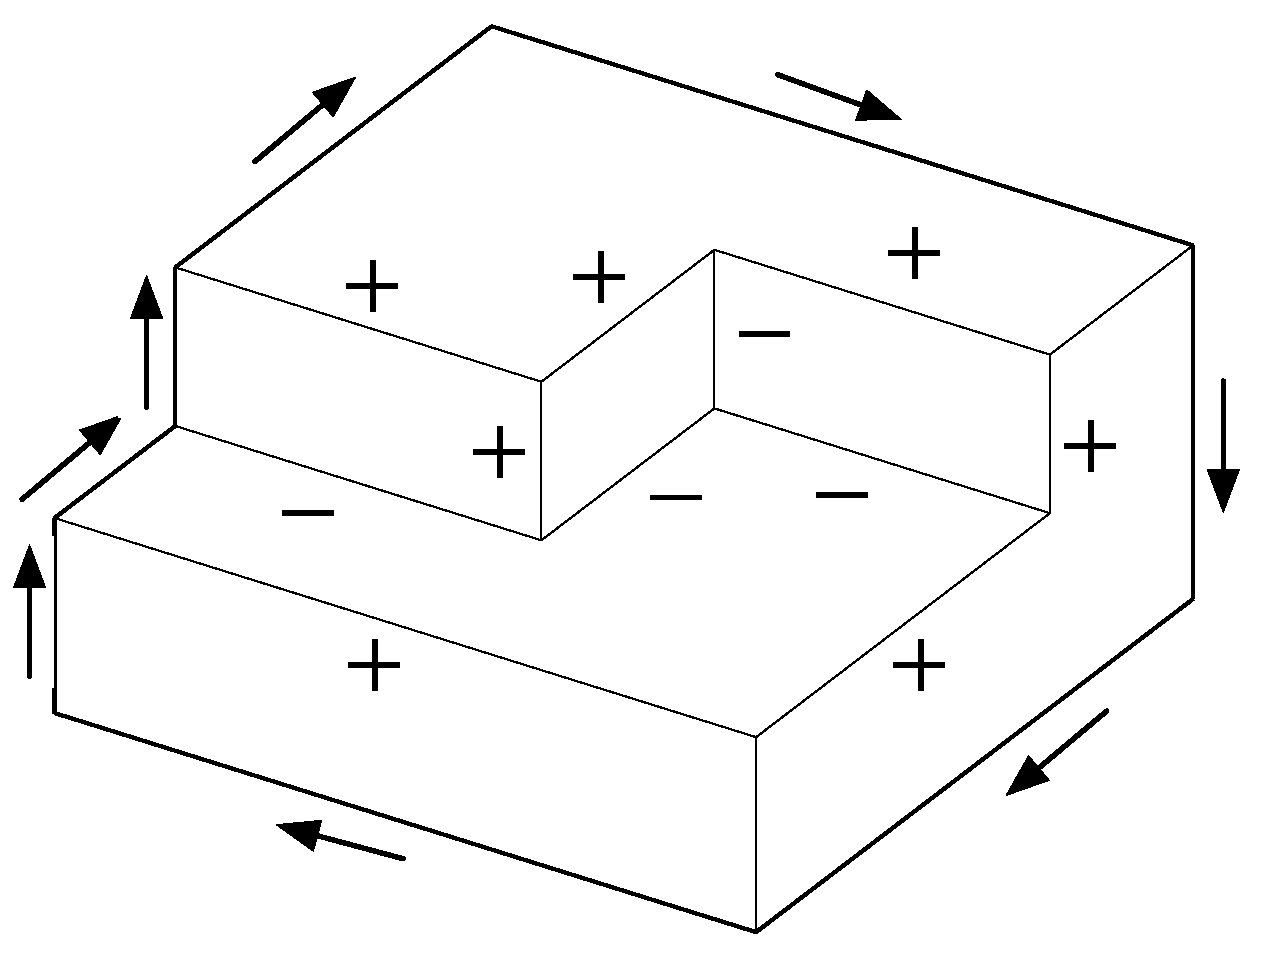
\includegraphics[origin=c,width=2in]{img/huffman-clowes.pdf} \caption{An
   illustration of Huffman-Clowes labels. Arrows indicate edges whose
   faces are obscured.  $+$ and $-$ identify edges as convex and
   concave.}  
   \label{fig:huffman-clowes} }
\end{center}
\end{figure}

3D recognition begins much the same way as 2D recognition. Individual
marks constituting a drawing are classified into features such as
lines, curves, and junctions. The recognizer must determine the
relationship between these features. For example, if a line represents
an edge between two faces, what is the dihedral angle?  There are a
number of ways to perform this analysis. Two are discussed briefly
below.

One approach to 3D stroke analysis is to label drawn and emergent
elements such as lines, vertices, and faces. The Huffman-Clowes
method~\cite{clowes-seeing-things,huffman-nonsense} identifies various
ways faces of a drawn polyhedron may relate (see
Figure~\ref{fig:huffman-clowes}). This helps reconstruct the 3D
geometry of the object based on the 2D drawing. A Huffman-Clowes label
indicates whether the line represents a concave or convex edge. Edges
are labeled ``obscuring'' if one of the adjoining faces is not
visible. Given a line drawing, there may be more than one possible way
to assign Huffman-Clowes labels~\cite{thorpe_huffman_clowes} (see
Figure~\ref{fig:necker}). Schweikardt and Gross used Huffman-Clowes to
interpret sketches of 3D objects in their Digital Clay
system~\cite{schweikardt-digital-clay}.

Shpitalni and Lipson use regression to classify input strokes and
clustering to identify 3D vertices shared by multiple lines. Stroke
classification fits input to conic sections using a linear system of
equations~\cite{shpitalni-curve-fitting}.  This approach is effective
for detecting straight lines, parabolic arcs, and hyperbolae. A sharp
(or filleted) corner, for example, can be found with a hyperbolic
conic section. After detecting curves, neighboring curve endpoints are
merged when appropriate.

\begin{figure}
\begin{center}
\subfigure[] { 
  \label{fig:necker-wireframe}
  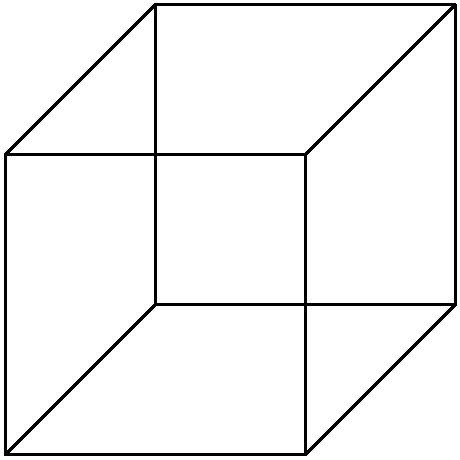
\includegraphics[origin=c,width=0.8in]{img/necker-wireframe-only.pdf}
}
\subfigure[] { 
  \label{fig:necker-interp-a}
  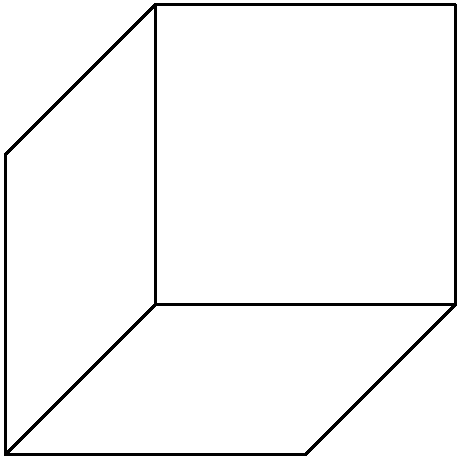
\includegraphics[origin=c,width=0.8in]{img/necker-interp-a.pdf}
}
\subfigure[] { 
  \label{fig:necker-interp-b}
  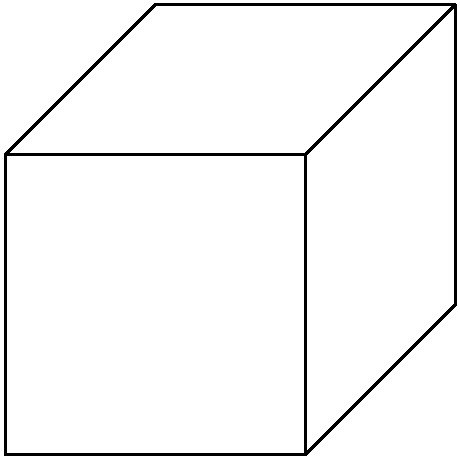
\includegraphics[origin=c,width=0.8in]{img/necker-interp-b.pdf}
}
\caption{A Necker Cube illustrates difficulty when forming 3D 
         interpretations of 2D line drawings. The wireframe shown
         in \subref{fig:necker-wireframe} can be interpreted in two
         equally valid ways, shown in \subref{fig:necker-interp-a}
         and \subref{fig:necker-interp-b} with hidden edges removed.}.
\label{fig:necker}
\end{center}
\end{figure}

\subsection{Gesture-based 3D recognition}

One way to provide input for a 3D sketching system is gestural
commands for creating or editing solid geometry models.
SKETCH~\cite{zeleznik-sketch} and
SKETCH-N-MAKE~\cite{bloomenthal-sketch-n-make} recognize gestural
commands to represent certain 3D forms. For example, when the user
draws two parallel lines, the system generates a cylinder. The drawing
direction defines whether the solid is additive (upward gestures) or
subtractive (downward gestures).

\subsection{Direct and indirect solid model drawing}

Teddy~\cite{igarashi-teddy} interprets user input as the outline of an
object. The object is then inflated to provide a smooth, blobby
object. Subsequent edits are done by explicitly changing modes and
entering commands as appropriate. For example, an object in Teddy may
be extended by drawing an attachment point on the existing object
followed by an outline of the new part of the object.

Not all the user's marks denote object boundaries. Designers draw
shadows, stipple dots, or little lines to indicate curvature or
surface texture. Cohen leverages this to create 3D models from
sketches by drawing shadows of objects~\cite{cohen-3d}. In this
system, ink is interpreted either as solid model geometry or as
the \textit{shadow} of that geometry projected onto a floor plane
below.

\subsection{Imposing and Inferring 3D Axes}

Finding depth values for vertices in a 3D sketch is easier if the
drawing conforms to an axis system, and if the object's faces are
known to be generally parallel to these axes. It may be reasonable to
impose a 3D axis scheme on the user. Alternately, the system can
interpret a user's drawing and infer an axis system.

Chateau allows people to design 3D objects (like French villa-style
buildings) using a constrained vocabulary of lines and
angles~\cite{igarashi-suggestive}. In Chateau, ink is interpreted as
wireframe elements that may connect to existing pieces on an explicit
``drawing plane''.

A coordinate system helps orient the user's marks so the overall
geometry can be found. However, some 3D sketching systems do not
provide a default 3D axis. The user may draw objects from any
perspective. One approach forms an Angular Distribution Graph (ADG)
showing how often lines are drawn at each
angle~\cite{lipson-correlation,masry-3d-sketch}. The ADG allows the
software to infer a coordinate system based on an analysis of the
drawing itself.

Tsang presents two methods for guiding 3D
reconstruction~\cite{tsang-3d-sketching}. In their system, recognition
works in the context of two kinds of guides. First, a 2D image may be
imported and placed in the drawing environment. The position and
curvature of sketched input is influenced by these images. Second, the
system analyses the drawing and suggests 3D wireframe models from a
database composed of prior work by the user or by third parties.

\subsection{Styling based on existing 3D geometry}

In many three-dimensional sketching systems, the visual representation
is often beautified during reconstruction from 2D to
3D. Beautification may substantially change the character of the
drawing so it no longer looks ``sketchy''. 

The work by Nealen and colleagues builds on the Teddy-like approach of
generating smooth 3D objects based on a
sketch~\cite{nealen-3d-sketch,nealen-fibermesh}. Users may draw on the
surface of 3D objects as a way to issue modeling commands. To stretch
a region of interest, the user first draws on the object to create the
control points, then drags them to stretch the surface.

Often designers create new instances of known object types. For
example, when designing the shape of computer speakers, designers work
from experience with other speakers. By providing a 3D wireframe that
is approximately the same shape as the desired object, a designer can
sketch around the wireframe to create a new
shape~\cite{mitani-3d-sketch,kara-3d-styling}. The user's marks are
recognized in the context of the wireframe, enabling the designer to
quickly create a new styled instance of an existing class of objects
without having to first make the wireframe.

A related approach is shown in the domain of organic plant
modeling~\cite{anastacio-plant-sketching}. Instead of a geometric
wireframe, this approach applies a mathematical model specifying the
target domain based on knowledge of plant biology. This technique
allows designers to quickly converge on a specific, highly refined 3D
model by sketching. To be sure, this advantage comes at the cost of
generality.

\section{Recognition training and domain modeling}
\label{sec:recognition-training}

In order for a sketch recognizer to interpret user input it first
needs a representation of whatever elements it is intended to
identify. There are two broad categories of methods for acquiring the
model from users. The first is to provide drawn examples; the second
is to provide written descriptions.

Many of the pattern recognizers discussed here provide user interfaces
for capturing training examples. In general these all work the same
way: users provide pen input and then label that input. The Rubine
recognizer and Quill require multiple training examples to determine
which analyzed features should be used to classify candidate input.

An alternative approach to providing drawn examples is to describe
symbols with some sort of text
description~\cite{mas-graph-grammar}. Costagliola \textit{et. al}
refer to these as \textit{Sketch Grammars}, or SkGs for
short~\cite{costagliola-skg}. A SkG is a BNF-like description of how
low-level elements like lines and circles can combine to form
higher-level elements. The combinations are described in terms of
geometric shapes and constraints describing their relative lengths,
positions, and angles. Once an entity's grammar is defined it may be
used to compose more complex elements. The grammar-based recognition
approaches covered here all share similar constraint types such
as \textit{parallel}, \textit{perpendicular}, \textit{above},
\textit{below}, \textit{smaller-than}, and \textit{centered-inside}.

Current work on sketch parsing leverages prior work from the visual
languages community. Lakin describes visual language parsing as ``the
process of recovering the underlying syntactic structure of a visual
communication object from its spatial arrangement.'' Lakin's vmacs
system~\cite{lakin-vmacs-89} supports users in providing unstructured
graphic input that can optionally be parsed by a visual grammar in
order to formally describe the structure of the depiction.

Grammar-based diagram parsing by Futrelle and Nikolakis focused on
parsing scientific figures as they appear in
publications~\cite{futrelle-diagram-parsing}. This research used
vector graphics rather than rough sketches, but it could be applied to
interpreting hand-drawn diagrams.

Compound objects were defined in the Electronic Cocktail Napkin (ECN)
as a set of elements and spatial relations~\cite{gross-boe}. The ECN
generated symbolic constraint descriptions from the user's sketch
input. The user could then modify the description by adding or
deleting constraints, or generalizing or making them more
specific. The ECN used a hybrid recognition approach involving a
low-level pattern-based recognizer to identify symbols and a
high-level grammar-based approach to recognize pattern configurations.

Constraints are often used to prescribe relations between elements
during design (``ensure line A remains perpendicular to line B, even
if line B moves''). But constraints may also be used to describe
relations exhibited by recognizable elements. Rather than using
constraints as rules for enforcing some conditions, they can be used
to search for configurations that match known elements. Pasternak's
ADIK system searches constraint declarations as a method for
performing diagram recognition~\cite{pasternak-adik}. To use the above
example, a user may define a plus symbol using constraints such as
``line A is perpendicular to line B''. Other constraints would specify
the relative size and positions. ADIK constraints also specify
tolerances so hand-made drawings could be recognized.

Hammond's LADDER language~\cite{hammond-ladder} builds on work
pioneered by systems like ADIK by enabling users to textually describe
how domain elements are drawn by stating the element composition and
constraints governing those elements. LADDER allows programmers to
prescribe how the element should be recognized, displayed, and how
users could interact with the elements once recognized. For example,
an object's ``editing'' definition may specify whether an object may
be rotated.

Recognizers like Ledeen or Rubine learn based on drawn examples. A
challenge with those approaches is that they must determine which
features of the drawing are important and which are not, generally
without user assistance. The salient features are extracted from
training examples. Grammar-based approaches may be difficult to write,
especially if recognizable classes have visual features that are
cumbersome to describe verbally. After all, drawings (sometimes)
encode nuances that are difficult to describe in words.

A third approach builds on the two others described above by combining
the benefits of grammatical descriptions with drawn examples. Shilman
describes a system similar to LADDER that incorporates the use of a
statistical model for parameterizing the spatial relations between
drawn elements~\cite{shilman-parsing}. Typically, a relationship such
as ``A is directly above B'' is interpreted as either \textit{true}
or \textit{false} based on some threshold values that give definition
for the word \textit{directly}. Shilman's approach allows the system
to learn statistical distributions based on training set examples. In
this case, the statement ``A is directly above B'' can take on various
levels of truth. Shilman uses a labeling scheme based on a na\"ive
Bayesian classifier.

Another hybrid approach involves generating grammars based on analysis
of
sketches~\cite{veselova-perceptual,hammond-interactive-descriptions}. Users
provide either a sketch or a textual description of a new element to
recognize. The system then generates a shape that is close to (a
``near miss'') the user's original input. The user then adds or
removes constraints as necessary to improve the match. This iterative
process of shape generation and constraint refinement continues until
the system produces a satisfactory model from the description of
constraints.

\vspace{12pt}

This section has discussed several aspects of sketch
recognition, including when, what, and how much to
recognize. Algorithms for segmentation and reasoning have also been
reviewed. Last, we described approaches for training recognition
systems to learn symbols, make use of contexts, and understand domain
semantics. The challenges in this section are primarily technical. The
following section continues the topic of sketch recognition from the
perspective of human interaction.
